\chapter{Kinematics for NAO: Our approach}
\label{approach}
As we mentioned before, there are already solutions for both problems but none of them is completely suitable for our needs. We want to be able to find a solution to the forward kinematics problem with any joint values for input and not only with the current values of the joint of NAO. Also, we need a real-time analytical solution for the problem of inverse kinematics without any approximations. Below we will describe our solutions for both of these problems.
\section{Forward Kinematics for the NAO Robot}
Aldebaran provides us with the DH parameters for each kinematic chain of the robot. The problem is that for some chains the given parameters are incorrect. More specifically, the parameters for the NAO arms are incorrect, so we found our own parameters for the arms and we used the parameters that Aldebaran gave us for the legs and the head.\\
\\

\textbf{NAO Zero Position}\\
We must define the base frame of the NAO and the zero position before we continue to the solution. First, the base frame is the torso frame and in the figure~\ref{fig:torso} we can see the axis of this frame. In this figure we can also see the zero position of the robot. As we can see, in this position the shoulder roll is not a roll joint but is a yaw joint, so we can understand that the names of the motors doesn't describe the correct movement of the joint.

\begin{figure}[h]
	\begin{center}
		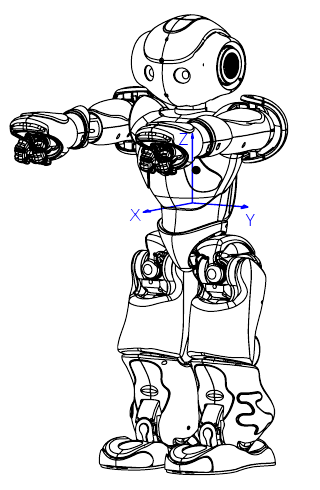
\includegraphics[height = 10cm]{Figures/torso_frame.png}
 		\caption{Torso Frame}
 		\label{fig:torso}
	\end{center}
\end{figure}


\textbf{Symbols}\\
We are going to give a simple explanation to the symbols that we are using for our math calculations. First of all, all the matrices that we are using are affine transformation matrices. Second, we have three types of matrices: \(T,R,A\). \(T\) is the transformation matrix, \(R_x, R_y, R_z\) are the basic rotations matrices and \(A\) is the translation matrix. The subscript of the symbol refers to the start frame and the superscript refers to the destination frame. The torso is the point that all the kinematic chains start and it is located on the center of the body of NAO. 'Base' will be the start frame and so will be the torso, and 'End' will be the end effector. The numbers will refer to one of the joints of the kinematic chain, as we see in the tables in Chapter~\ref{problem}. Also, we define the initialization of the translation matrix as: \(A(d_x,d_y,d_z)\) and for the rotation matrices as: \(R_x(\theta_x) \text{ or } R_y(\theta_y) \text{ or } R_z(\theta_z)\).\\
We will present the DH parameters in tables and except from the DH parameters, in the tables we will have the translations from the base to the first joint and from the last joint to the end effector. Also, we will have some necessary rotations to adjust the frame of the last joint to the frame of the end effector.\\
\\

\textbf{Forward Kinematics equations}\\
Forward kinematics for each chain of the NAO robot is an equation that transforms a point from the frame of the last joint to the base frame. In our case we will have an end effector that will be the point of interest. So, we can construct these equations with the use of transformation, rotation and translation matrices.\\

\textbf{Extracting the position}\\
As we will see, the result of forward kinematics is an affine transformation matrix with \(X\) submatrix to be a rotation matrix and \(Y\) a translation vector. We need to extract the \(p_x,p_y\) and \(p_z\) points and the \(a_x,a_y\) and \(a_z\) angles of the final position. So, we can extract \(p_x,p_y\) and \(p_z\) from the translation part of the matrix:
\begin{small}
\begin{align*}
p_x &= T_{(1,4)}\\
p_y &= T_{(2,4)}\\
p_z &= T_{(3,4)}
\end{align*}
\end{small}

Now we must extract the \(a_x,a_y\) and \(a_z\) from the rotation table. The rotation of the final transformation table is a \(R_zR_yR_z\) rotation table. In chapter '2' we present the analytical form of this table. Now it's easy to extract the angles:
\begin{small}
\begin{align*}
a_x &= \arctan2\left(T_{(3,2)},T_{(3,3)}\right)\\
a_y &= \arctan2\left(-T_{(3,1)},\sqrt{T^2_{(3,2)} + T^2_{(3,3)}}\right)\\
a_z &= \arctan2\left(T_{(2,1)},T_{(1,1)}\right)
\end{align*}
\end{small}

\subsection{Forward Kinematics for the Head}
The head of NAO is the simplest kinematic chain but, it has two possible end effectors, the top and the bottom camera position on the head. As we will see in our solution, it is easy to change the end effector by just changing the last translation matrix. Below, there is the table with all the DH parameters for this chain and the two possible end effectors. \\
\begin{table}[h]
\centering
\begin{tabular}{|l|>{\centering\arraybackslash}m{2.55cm}|>{\centering\arraybackslash}m{2.55cm}|>{\centering\arraybackslash}m{2.55cm}|>{\centering\arraybackslash}m{2.55cm}|}
\hline
\textbf{Frame (Joint)} & \(\mathbf{a}\) & \(\boldsymbol{\alpha}\) & \(\mathbf{d}\) & \(\boldsymbol{\theta}\)\\ \hline
Base & \multicolumn{4}{c|}{\(A(0,0,\text{\footnotesize{NeckOffsetZ}})\)} \\ \hline
HeadYaw & \(0\) & \(0\) & \(0\) & \(\theta_1\) \\ \hline
HeadPitch & \(0\) & \(-\frac{\pi}{2}\) & \(0\) & \(\theta_2 - \frac{\pi}{2}\) \\ \hline
Rotation & \multicolumn{4}{c|}{\(R_x(\frac{\pi}{2})R_y(\frac{\pi}{2})\)} \\ \hline
Top Camera & \multicolumn{4}{c|}{\(A(\text{\footnotesize{topCameraX}},0,\text{\footnotesize{topCameraZ}})\)} \\ \hline
Bottom Camera & \multicolumn{4}{c|}{\(A(\text{\footnotesize{bottomCameraX}},0,\text{\footnotesize{bottomCameraZ}})\)} \\ \hline
\end{tabular}
\caption{DH parameters for Head chain}
\label{tab:DH parameters for Head chain}
\end{table}

Now we can combine the tables and find the point of the end effector in the frame space of the torso:
\[
T^\text{End}_\text{Base} = A^0_\text{Base}T^1_0T^2_1R_x(\tfrac{\pi}{2})R_y(\tfrac{\pi}{2})A^\text{End}_{2}
\]
The DH transformation matrices are \(T^1_0\text{ and }T^2_1\). The translation of the end effector can be replaced by one of the two possible translation matrices. Now we have the position of the end effector in the \(three-dimensional\) space of the torso.

\subsection{Forward Kinematics for the Left Arm}
Aldebaran's give a set of DH parameters for the arms, but after the implementation of forward kinematics with these parameters we observed that the output was incorrect. So we find our own set of DH parameters for the arms of the robot.\\
The kinematic chain for the left arm consists of four joints. So we need to find four sets of DH parameters, one set for every joint. First we must move from the torso to the base of the joint and we can do that with a simple translation. After that we must align the coordinate frame rotation axis of the joint. So we are rotate the \(x\)-axis (the $\alpha$ parameter) of the system by \(-\frac{\pi}{2}}. Now we must rotate again the coordinate frame to become aligned with the rotation axis of the second joint. So, now we rotate the \(x\)-axis by \(\frac{\pi}{2}}. Next, we will need to align the coordinate system with the rotation axis of the third joint. Now, to align the coordinate system we must rotate the \(y\)-axis. The DH parameters doesn't implement a rotation by the \(y\)-axis, so, we must first rotate the \(z\)-axis and then the \(x\)-axis. These two rotations can simulation a \(y\)-axis rotation. Thus, we must subtract \(-\frac{\pi}{2}} from the \(\theta\) of the previous joint and rotate the \(x\)-axis by \(-\frac{\pi}{2}}. Then, we must move toward \(z\)-axis to reach the position of the joint, so, \(d\) parameter equals UpperArmLength. Finally, for the last joint we rotate the \(x\)-axis by \(\frac{\pi}{2}}. Now, we need only a rotation to fix the orientation of our coordinate system and a translation to reach the end effector.\\
Below we can see the table with the DH parameters for all joints and with the necessary translations and rotations.
\begin{table}[!h]
\centering
\begin{tabular}{|l|>{\centering\arraybackslash}m{2.55cm}|>{\centering\arraybackslash}m{2.55cm}|>{\centering\arraybackslash}m{2.55cm}|>{\centering\arraybackslash}m{2.55cm}|}
\hline
\textbf{Frame (Joint)} & \(\mathbf{a}\) & \(\boldsymbol{\alpha}\) & \(\mathbf{d}\) & \(\boldsymbol{\theta}\)\\ \hline
Base & \multicolumn{4}{|c|}{\(A(0,\text{\footnotesize{ShoulderOffsetY+ElbowOffsetY}},\text{\footnotesize{ShoulderOffsetZ}})\)} \\ \hline
LShoulderPitch & \(0\) & \(-\frac{\pi}{2}\) & \(0\) & \(\theta_1\) \\ \hline
LShoulderRoll & \(0\) & \(\frac{\pi}{2}\) & \(0\) & \(\theta_2 - \frac{\pi}{2}\) \\ \hline
LElbowYaw & \(0\) & \(-\frac{\pi}{2}\) & \footnotesize{UpperArmLength} & \(\theta_3\) \\ \hline
LElbowRoll & \(0\) & \(\frac{\pi}{2}\) & \(0\) & \(\theta_4\) \\ \hline
Rotation & \multicolumn{4}{c|}{\(R_z(\frac{\pi}{2})\)} \\ \hline
End effector & \multicolumn{4}{c|}{\(A(\text{\footnotesize{HandOffsetX+LowerArmLength}},0,0)\)} \\ \hline
\end{tabular}
\caption{DH parameters for Left Arm chain}
\label{tab:DH parameters for Left Arm chain}
\end{table}
Now we can easily calculate the final transformation table:
\[
T^\text{End}_\text{Base} = A^0_\text{Base}T^1_0T^2_1T^3_2T^4_3R_z(\tfrac{\pi}{2})A^\text{End}_{4}
\]
The DH transformation matrices are the \(T^1_0,T^2_1,T^3_2\text{ and }T^4_3\). Now we have the transformation table for the position of the end effector of the left arm relatively to the frame of the torso.

\subsection{Forward Kinematics for the Right Arm}
The kinematic chain of the right arm is symmetric with the chain of the left arm relatively to the plain defined by \(x\) and \(z\)-axis. So, the differences with the left arm will be only in the distances along \(y\)-axis and in the joints that move the \(y\)-axis (angle roll joints). Also, in this chain we must add one extra rotation matrix after the final translation, because the \(z\)-axis is inverted.
\begin{table}[!h]
\centering
\begin{tabular}{|l|>{\centering\arraybackslash}m{2.55cm}|>{\centering\arraybackslash}m{2.55cm}|>{\centering\arraybackslash}m{2.55cm}|>{\centering\arraybackslash}m{2.55cm}|}
\hline
\textbf{Frame (Joint)} & \(\mathbf{a}\) & \(\boldsymbol{\alpha}\) & \(\mathbf{d}\) & \(\boldsymbol{\theta}\)\\ \hline
Base & \multicolumn{4}{|c|}{\(A(0,\text{\footnotesize{-ShoulderOffsetY - ElbowOffsetY}},\text{\footnotesize{ShoulderOffsetZ}})\)} \\ \hline
RShoulderPitch & \(0\) & \(-\frac{\pi}{2}\) & \(0\) & \(\theta_1\) \\ \hline
RShoulderRoll & \(0\) & \(\frac{\pi}{2}\) & \(0\) & \(\theta_2 + \frac{\pi}{2}\) \\ \hline
RElbowYaw & \(0\) & \(-\frac{\pi}{2}\) & \footnotesize{-UpperArmLength} & \(\theta_3\) \\ \hline
RElbowRoll & \(0\) & \(\frac{\pi}{2}\) & \(0\) & \(\theta_4\) \\ \hline
Rotation & \multicolumn{4}{c|}{\(R_z(\frac{\pi}{2})\)} \\ \hline
End effector & \multicolumn{4}{c|}{\(A(\text{\footnotesize{-HandOffsetX-LowerArmLength}},0,0)\)} \\ \hline
Rotation$^{'}$ & \multicolumn{4}{c|}{\(R_z(-\pi)\)} \\ \hline
\end{tabular}
\caption{DH parameters for Right Arm chain}
\label{tab:DH parameters for Right Arm chain}
\end{table}
\[
T^\text{End}_\text{Base} = A^0_\text{Base}T^1_0T^2_1T^3_2T^4_3R_z(\tfrac{\pi}{2})A^\text{End}_{4}R_z(-\pi)
\]
The DH transformation matrices are the \(T^1_0,T^2_1,T^3_2\text{ and }T^4_3\). Now we have the transformation table for the position of the end effector of the right arm relatively to the frame of the torso.

\subsection{Forward Kinematics for the Left Leg}
The kinematic chain for the left leg has six joints and it is the biggest chain on the NAO. The DH parameters of these joints are slightly different because of the YawPitch joint.
\begin{table}[!h]
\centering
\begin{tabular}{|l|>{\centering\arraybackslash}m{2.55cm}|>{\centering\arraybackslash}m{2.55cm}|>{\centering\arraybackslash}m{2.55cm}|>{\centering\arraybackslash}m{2.55cm}|}
\hline
\textbf{Frame (Joint)} & \(\mathbf{a}\) & \(\boldsymbol{\alpha}\) & \(\mathbf{d}\) & \(\boldsymbol{\theta}\)\\ \hline
Base & \multicolumn{4}{|c|}{\(A(0,\text{\footnotesize{HipOffsetY}},\text{\footnotesize{-HipOffsetZ}})\)} \\ \hline
LHipYawPitch & \(0\) & \(-\frac{3\pi}{4}\) & \(0\) & \(\theta_1 - \frac{\pi}{2}\) \\ \hline
LHipRoll & \(0\) & \(-\frac{\pi}{2}\) & \(0\) & \(\theta_2 + \frac{\pi}{4}\) \\ \hline
LHipPitch & \(0\) & \(\frac{\pi}{2}\) & \(0\) & \(\theta_3\) \\ \hline
LKneePitch & \footnotesize{-ThighLength} & \(0\) & \(0\) & \(\theta_4\) \\ \hline
LAnklePitch & \footnotesize{-TibiaLength} & \(0\) & \(0\) & \(\theta_5\) \\ \hline
LAnkleRoll & \(0\) & \(-\frac{\pi}{2}\) & \(0\) & \(\theta_6\) \\ \hline
Rotation & \multicolumn{4}{c|}{\(R_z(\pi)R_y(-\tfrac{\pi}{2})\)} \\ \hline
End effector & \multicolumn{4}{c|}{\(A(0,0,\text{\footnotesize{-FootHeight}})\)} \\ \hline
\end{tabular}
\caption{DH parameters for Left Leg chain}
\label{tab:DH parameters for Left Leg chain}
\end{table}
\[
T^\text{End}_\text{Base} = A^0_\text{Base}T^1_0T^2_1T^3_2T^4_3T^5_4T^6_5R_z(\pi)R_y(-\tfrac{\pi}{2})A^\text{End}_{6}
\]
The DH transformation matrices are the \(T^1_0,T^2_1,T^3_2,T^4_3,T^5_4\text{ and }T^6_5\). Now we have the transformation table for the position of the end effector of the left leg relatively to the frame of the torso.

\subsection{Forward Kinematics for the Right Leg}
As for the hands, the kinematic chains for the legs are symmetric relatively to the plain defined by \(x\) and \(z\)-axis. So, the differences of the chain for the right leg will be only in the distances along \(y\)-axis and in the joints that move the \(y\)-axis.
\\
\\
\\
\begin{table}[!h]
\centering
\begin{tabular}{|l|>{\centering\arraybackslash}m{2.55cm}|>{\centering\arraybackslash}m{2.55cm}|>{\centering\arraybackslash}m{2.55cm}|>{\centering\arraybackslash}m{2.55cm}|}
\hline
\textbf{Frame (Joint)} & \(\mathbf{a}\) & \(\boldsymbol{\alpha}\) & \(\mathbf{d}\) & \(\boldsymbol{\theta}\)\\ \hline
Base & \multicolumn{4}{|c|}{\(A(0,\text{\footnotesize{-HipOffsetY}},\text{\footnotesize{-HipOffsetZ}})\)} \\ \hline
RHipYawPitch & \(0\) & \(-\frac{\pi}{4}\) & \(0\) & \(\theta_1 - \frac{\pi}{2}\) \\ \hline
RHipRoll & \(0\) & \(-\frac{\pi}{2}\) & \(0\) & \(\theta_2 - \frac{\pi}{4}\) \\ \hline
RHipPitch & \(0\) & \(\frac{\pi}{2}\) & \(0\) & \(\theta_3\) \\ \hline
RKneePitch & \(-ThighLength\) & \(0\) & \(0\) & \(\theta_4\) \\ \hline
RAnklePitch & \(-TibiaLength\) & \(0\) & \(0\) & \(\theta_5\) \\ \hline
RAnkleRoll & \(0\) & \(-\frac{\pi}{2}\) & \(0\) & \(\theta_6\) \\ \hline
Rotation & \multicolumn{4}{c|}{\(R_z(\pi)R_y(-\tfrac{\pi}{2})\)} \\ \hline
End effector & \multicolumn{4}{c|}{\(A(0,0,\text{\footnotesize{-FootHeight}})\)} \\ \hline
\end{tabular}
\caption{DH parameters for Right Leg chain}
\label{tab:DH parameters for Right Leg chain}
\end{table}
\[
T^\text{End}_\text{Base} = A^0_\text{Base}T^1_0T^2_1T^3_2T^4_3T^5_4T^6_5R_z(\pi)R_y(-\tfrac{\pi}{2})A^\text{End}_{6}
\]
The DH transformation matrices are the \(T^1_0,T^2_1,T^3_2,T^4_3,T^5_4\text{ and }T^6_5\). Now we have the transformation table for the position of the end effector of the right leg relatively to the frame of the torso.

\subsection{Forward Kinematics for merged chains}
We have found the solution only for the chains that have as base frame the torso frame. In the real word, someone maybe wants to find the torso position relatively to one of the feet chains. If we get the final transformation table for, e.g., the left leg, we know that it is an affine transformation matrix and because of that, we can invert the table and then we will have the position of the torso relatively to the frame of the left leg. 
\[
T^\text{Torso}_\text{Lleg} = {\left(T^\text{Lleg}_\text{Torso}\right)}^{-1}
\]
Also, it is possible to find the position of the head relatively to the left leg. The kinematic chains for the head and for the left leg are relative to the torso frame. So, if we invert the chain of the left leg, we will have the torso relatively to the left leg frame. Then we can just multiply the transformation table that has the position of the head relatively to the torso frame and we will have the position of the head relatively to the left leg frame.
\[
T^\text{Head}_\text{Lleg} = {\left(T^\text{Lleg}_\text{Torso}\right)}^{-1}T^\text{Head}_\text{Torso}
\]
This property is very useful, because we can find any end effector relatively to any other end effector. For example, with this, we can find the height of the camera from the ground.

\subsection{Calculation of Center Of Mass with Forward Kinematics}
The calculation of the center of mass (CoM) is very important because NAO consists of a group of moving parts. Every moving part has a mass and with forward kinematics we can calculate the position of the CoM relatively to a given frame. Aldebaran provides us with the whole information that is needed to do the calculation. Aldebaran gives us the mass of the whole robot and the mass for every moving part of NAO. The separate masses are given according to every joint of the robot. Thus, every joint of the robot has a mass and the position of the CoM for this joint relatively to the joint frame.\\
The CoM is calculated relatively to the torso frame and the calculation order is simple. We construct smaller kinematic chains that stop to an earlier joint, and then we set as the end effector the position of CoM for the frame of the joint where we stop. Then we get the translation part and we multiply it by the mass of the certain part. At the end, we will have 21 chains plus the torso chain. Then we will add all the individual translation matrices that have been weighted by the mass of each joint and the result will be divided by the total mass. The result will be the position of the CoM relatively to the torso frame.



\section{Inverse Kinematics for NAO}
Forward kinematics can find the position of an end effector, relatively to the start frame, given the joints values. Now we have to solve the inverse problem: find the joints values given the desired end effector position relatively to the torso frame. The solutions for the inverse kinematics problem that will be presented below are related to the kinematic chains that start from the torso.\\
The position of the end effector is the \(p_x,p_y\text{ and }p_z\) points along with the \(a_x,a_y\text{ and }a_z\) angles. As we mentioned before, the product of forward kinematics is an affine transformation matrix and it consists of a rotation and a translation matrix. The rotation \(R\) is equal to \(R_zR_yR_x\). Thus, we can construct the transformation table:

\begin{scriptsize}
\[
T = 
\begin{bmatrix}
\cos a_y\cos a_z & -\cos a_x\sin a_z + \sin a_x\sin a_y\cos a_z & \sin a_x\sin a_z + \cos a_x\sin a_y\cos a_z & p_x\\
\cos a_y\sin a_z & \cos a_x\cos a_z + \sin a_x\sin a_y\sin a_z & -\sin a_x\cos a_z + \cos a_x\sin a_y\sin a_z & p_y\\
-\sin a_y & \sin a_x\cos a_y & \cos a_x\cos a_y & p_z\\
0 & 0 & 0 & 1
\end{bmatrix}
\]
\end{scriptsize}\\
As we mentioned before we can't solve the problem of inverse kinematics without the solution of forward kinematics. That's why the equations that we must solve to find the values of joints are the matrices from the forward kinematics but with the \(\theta\) from DH parameters as the unknown part. So, we can find the symbolic table that is the product of forward kinematics and equate it with the matrix above. Then, we will have twelve equations (we don't have sixteen because the last line of the matrix is always (\(0\) \(0\) \(0\) \(1\))) and \(n\) unknowns, where \(n\) is the number of joints in the chain. In fact, we will have \(2n\) unknowns, because all the thetas (\(\theta\)) appear inside \(\sin\) or \(\cos\).\\
As we will see below, we found some of the desired angles with \(\arccos \text{ and }\arcsin\). The problem is that \(\arcsin\) returns a number in \(\left[-\tfrac{\pi}{2},\tfrac{\pi}{2}\right]\) and \(\arccos\) returns a number in \(\left[0,\pi\right]\) but the possible range of the joints is in \(\left[-\pi,\pi\right]\). Thus, we will have two possible solutions for every \(\arcsin\) and \(\arccos\) (because of the complimentary angles). Because of that, we must filter our results and keep only the correct angles. We achieve that by doing a forward validation step when we find a complete set of angle values. Then we compare the result of the validation step with the reconstructed table and if they are equal, then we approve the set. Some complimentary angles will be discarded a long time before the validation step due to the range restriction of each joint.

\subsection{Inverse Kinematics for the Head}
The head chain, as we said before, consists only of two joints. Thus, we can find both desired angles only by the \(a_z\) and \(a_y\). On the other hand, someone maybe wants to find the joints for the desired position by only using the target points \(p_x,p_y\text{ and }p_z\), so we implement another solution that works only with the target points. Below we can see the symbolic result from forward kinematics:
\[
T = 
\begin{bmatrix}
-\cos\theta_1\sin\theta_2 & -\sin\theta_1 & \cos\theta_1\cos\theta_2 &  l_2\cos\theta_1\cos\theta_2 - l_1\cos\theta_1\sin\theta_2\\
-\sin\theta_1\sin\theta_2 & \cos\theta_1 & \cos\theta_2\sin\theta_1 & l_2\cos\theta_2\sin\theta_1 - l_1\sin\theta_1\sin\theta_2\\
-\cos\theta_2 & 0 & -\sin\theta_2 & l_3 - l_2\sin\theta_2 - l_1\cos\theta_2\\
0 & 0 & 0 & 1
\end{bmatrix}
\]
where: \(l_1 = \text{cameraX, }l_2 = \text{cameraZ and }l_3 = \text{NeckOffsetZ}\).\\
Because we only know the \(p_x,p_y\text{ and }p_z\) and we can't reconstruct the rotation part of the matrix, we will only use the translation part that is reconstructed. Now we can see from the symbolic matrix that \(T_{(3,4)} = l_3 - l_2\sin\theta_2 - l_1\cos\theta_2 = p_z\) and we know from trigonometry that: 
\[
a\sin\theta + b\cos\theta = \sqrt{a^2+b^2}\sin\left(\theta + \psi\right)
\]
\[
\psi=\arctan\left(\frac{b}{a}\right) + \left\{ 
  \begin{array}{l l}
    0 & \quad \text{if }a\geq0\\
    \pi & \quad \text{if }a<0\\
  \end{array} \right.
\]
So, we can now calculate \(\theta_2\):
\[
\theta_2 = \arcsin\left(\cfrac{-p_z+l_3}{\sqrt{{l_1}^2+{l_2}^2}}\right) + \arctan\left(\frac{l_1}{l_2}\right)
\]
Now the final \(\theta_2\) is: \(\theta_2 = \theta_2 - \frac{\pi}{2}\) because in the DH parameters we had added \(\frac{\pi}{2}\) to the \(\theta\) parameter for the second joint.  From now on, we must substract \(\frac{\pi}{2}\) from \(\theta_2\) if we want to use it to calculate a result from the equations.\\
Then we can easily extract \(\theta_1\) from \(T_{(1,4)}\):
\[
\theta_1 = \arccos\left(\cfrac{p_x}{l_1\left(\theta_2 + \frac{\pi}{2}\right) - l_2\cos\left(\theta_2 + \frac{\pi}{2}\right)}\right)
\]
Finally, we must filter our results because of \(\arccos\text{ and }\arcsin\). So, we will do a forward kinematics validation set and we will discard any set of values that doesn't move the end effector to the correct position.\\
\\
So, the final inverse kinematics equations for the head are the following:\\
\begin{small}
\begin{align*}
%l_3 = neckoffset z
%l_1 = camera X
%l_2 = camera Z
\theta_2 &= \arcsin\left(\cfrac{- p_z + l_3}{ \sqrt{l^2_1 + l^2_2} }\right) + \frac{\pi}{2}\\
\theta_1 &= \arccos\left(\cfrac{p_x}{l_2\cos\left(\theta_2 - \frac{\pi}{2}\right) - l_1\sin\left(\theta_2 - \frac{\pi}{2}\right) } \right)
\end{align*}
\end{small}
or only with angles
\begin{small}
\begin{align*}
\theta_1 &= a_z\\
\theta_2 &= a_y
\end{align*}
\end{small}

\subsection{Inverse Kinematics for the Left Hand}
The left arm chain is far more complicated than the head chain. First, we must construct the symbolic matrix:\\
\begin{small}
\begin{align*}
T &= \begin{bmatrix}
r_{11} & r_{12} & r_{13} & r_{14}\\
r_{21} & r_{22} & r_{23} & r_{24}\\
r_{31} & r_{32} & r_{33} & r_{34}\\
0 & 0 & 0 & 1
\end{bmatrix}\\
r_{11} &= \sin\theta_4\left(\sin\theta_1\sin\theta_3 - \cos\theta_1\cos\theta_2\cos\theta_3\right) - \cos\theta_1\cos\theta_4\sin\theta_2\\
r_{12} &= \cos\theta_4\left(\sin\theta_1\sin\theta_3 - \cos\theta_1\cos\theta_2\cos\theta_3\right) + \cos\theta_1\sin\theta_2\sin\theta_4\\
r_{13} &= \cos\theta_3\sin\theta_1 + \cos\theta_1\cos\theta_2\sin\theta_3\\
r_{14} &= l_4\left(\sin\theta_4\left(\sin\theta_1\sin\theta_3 - \cos\theta_1\cos\theta_2\cos\theta_3\right) - \cos\theta_1\cos\theta_4\sin\theta_2\right) - l_3\cos\theta_1\sin\theta_2\\
r_{21} &= \cos\theta_2\cos\theta_4 - \cos\theta_3\sin\theta_2\sin\theta_4\\
r_{22} &= \cos\theta_2\sin\theta_4 - \cos\theta_3\cos\theta_4\sin\theta_2\\
r_{23} &= \sin\theta_2\sin\theta_3\\
r_{24} &= l_1 + l_3\cos\theta_2 + l_4\left(\cos\theta_2\cos\theta_4 - \cos\theta_3\sin\theta_2\sin\theta_4\right)\\
r_{31} &= \sin\theta_4\left(\cos\theta_1\sin\theta_3 + \cos\theta_2\cos\theta_3\sin\theta_1\right) + \cos\theta_4\sin\theta_1\sin\theta_2\\
r_{32} &= \cos\theta_4\left(\cos\theta_1\sin\theta_3 + \cos\theta_2\cos\theta_3\sin\theta_1\right) - \sin\theta_1\sin\theta_2\sin\theta_4\\
r_{33} &= \cos\theta_1\cos\theta_3 - \cos\theta_2\sin\theta_1\sin\theta_3\\
r_{34} &= l_2 + l_4\left(\sin\theta_4\left(\cos\theta_1\sin\theta_3 + \cos\theta_2\cos\theta_3\sin\theta_1\right) + \cos\theta_4\sin\theta_1\sin\theta_2\right) + l_3\sin\theta_1\sin\theta_2
\end{align*}
\end{small}\\
where: $l_1 =$ ShoulderOffsetY$+$ElbowOffsetY, $l_2 =$ ShoulderOffsetZ, $l_3 =$ UpperArmLength and $l_4 =$ HandOffsetX$+$LowerArmLength.\\
As we can see now, the problem of inverse kinematics for the arms is far more complicated than the problem for the head. It is very difficult to extract a joint value from all these equations, so, we can use trigonometry to find the value of one joint. More specifically this joint is the elbow roll joint. We can observe that the upper arm, the lower arm with the hand offset and the distance from the position of the shoulder pitch joint to the end effector forms a triangle and we know the size of each side. The position of the shoulder pitch joint relative to the torso frame is known, and the position of the end effector is the target position. So, the distance can be calculated:
\[
d=\sqrt{\left(s_x-p_x\right)^2 + \left(s_y-p_y\right)^2 + \left(s_z-p_z\right)^2}
\]
where: \(s_x = 0, s_y = l_1\) and \(s_z = l_2\).\\
Now we can use the cosine law and find \(\theta_4\):
\[
\theta_4 = \arccos\left(\frac{{l_3}^2 + {l_4}^2 - d^2}{2l_3l_4}\right)
\]
Because \(\theta_4\) represents an interior angle and the elbow roll joint is being stretched in the zero-position, the resulting angle is computed by:
\[
\theta_4 = \pi - \theta_4
\]
Because the \(\theta_4\) for the left arm take only negative values, we will take the \(-\theta_4\) so:
\[
\theta_4 = - \theta_4
\]
The next angle that we can find is the \(\theta_2\), so we can look for equations from the table symbolic matrix, where we only have \(\theta_2\) and one more unknown \(\theta\). Using $r_{22}$ we have:
\begin{small}
\begin{align*}
&T_{(2,2)} = -\cos\theta_2 - \cos\theta_3\cos\theta_4\sin\theta_2 &\Leftrightarrow\\
&\cos\theta_3\sin\theta_2 = -\cfrac{\cos\theta_2\sin\theta_4 + T_{(2,2)}}{\cos\theta_4}
\end{align*}
\end{small}\\
We can do the division because $\theta_4$ doesn't reach $\frac{\pi}{2} $ so, the cosine never becomes zero. Now we can go to $r_{24}$:
\begin{small}
\begin{align*}
&T_{(2,4)} = p_y = l_1 + l_3\cos\theta_2 + l_4\left(\cos\theta_2\cos\theta_4 - \cos\theta_3\sin\theta_2\sin\theta_4\right)&\Leftrightarrow\\
&p_y - l_1 =l_3\cos\theta_2 + l_4\cos\theta_2\cos\theta_4 - l_4\left(-\frac{\cos\theta_2\sin\theta_4 + T_{(2,2)}}{\cos\theta_4}\right)\sin\theta_4&\Leftrightarrow\\
&p_y - l_1 - \frac{l_4\sin\theta_4 T_{(2,2)}}{\cos\theta_4} = \cos\theta_2\left(l_3 + l_4\cos\theta_4 + l_4\frac{{\sin\theta_4}^2}{\cos\theta_4}\right)&\Leftrightarrow\\
&\theta_2 = \arccos\left(\cfrac{p_y - l_1 - \frac{l_4\sin\theta_4 T_{(2,2)}}{\cos\theta_4}}{l_3 + l_4\cos\theta_4 + l_4\frac{\sin^2\theta_4}{\cos\theta_4}}\right) \hspace{2cm} \text{because }   l_3 + l_4\cos\theta_4 + l_4\frac{\sin^2\theta_4}{\cos\theta_4}>0 \hspace{-0.8cm}
\end{align*}
\end{small}\\
Now the final \(\theta_2\) is: \(\theta_2 = \theta_2 + \frac{\pi}{2}\) because in the DH parameters we had added \(\frac{\pi}{2}\) to the \(\theta\) parameter for the second joint of the arm. From now on, we must substract \(\frac{\pi}{2}\) from \(\theta_2\) if we want to use it to calculate a result from the equations. Next we will calculate the $\theta_3$ angle:
\begin{small}
\begin{align*}
&T_{(2,3)} = \sin\left(\theta_2 - \frac{\pi}{2}\right)\sin\theta_3 &\Leftrightarrow \\
& \theta_3 = \arcsin\left( \cfrac{ T_{(2,3)} }{ \sin\left(\theta_2-\frac{\pi}{2}\right)}\right)  &\text{because }    \theta_2 \neq \left|\frac{\pi}{2}\right|
\end{align*}
\end{small}\\
Finally, we must extract the value for \(\theta_1\):
\begin{small}
\begin{align*}
&T_{(1,3)} = \cos\theta_3\sin\theta_1 + \cos\theta_1\cos\left(\theta_2 - \frac{\pi}{2}\right)\sin\theta_3 &\Leftrightarrow \\
&\sin\theta_1 = \cfrac{T_{(1,3)} - \cos\theta_1\cos\left(\theta_2 - \frac{\pi}{2}\right)\sin\theta_3}{\cos\theta_3}  &\text{when } \theta_3 \neq \left|\frac{\pi}{2}\right|\\
&\cos\theta_1 = \cfrac{T_{(1,3)}}{\cos\left(\theta_2 - \frac{\pi}{2}\right)\sin\theta_3}  &\text{when} \quad \theta_3 = \left|\frac{\pi}{2}\right|
\end{align*}
\end{small}\\
So, now we have two possible solutions for \(\theta_1\) and we choose between them depending on the value of \(\theta_3\). So, when $\theta_3 = \left|\frac{\pi}{2}\right|$:
\begin{small}
\begin{align*}
&\theta_1 = \arccos\left(\cfrac{T_{(1,3)}}{\cos\left(\theta_2 - \frac{\pi}{2}\right)\sin\theta_3}\right)
\end{align*}
\end{small}\\
Else if \(\theta_2 \neq \left|\frac{\pi}{2}\right|\), we will find the \(\theta_1\) from \(r_{33}\) and we will replace \(\sin\theta_1\) with the result above. So:
\begin{small}
\begin{align*}
&T_{(3,3)} = \cos\theta_1\cos\theta_3 - \cos\left(\theta_2 - \frac{\pi}{2}\right)\sin\theta_1\sin\theta_3 &\Leftrightarrow \\
&T_{(3,3)} = \cos\theta_1\cos\theta_3 - \left(\cfrac{T_{(1,3)} - \cos\theta_1\cos\left(\theta_2 - \frac{\pi}{2}\right)\sin\theta_3}{\cos\theta_3}\right)\sin\theta_3\cos\left(\theta_2 - \frac{\pi}{2}\right) &\Leftrightarrow \\
&\theta_1 = \arccos\left(\cfrac{T_{(3,3)} -\cfrac{ T_{(1,3)}\sin\theta_3\cos\left(\theta_2 - \frac{\pi}{2}\right)}{\cos\theta_3}}{\cos\theta_3 + \cfrac{\cos^2\left(\theta_2-\frac{\pi}{2}\right)\sin^2\theta_3}{\cos\theta_3}}\right)
\end{align*}
\end{small}\\
Now we have calculated all the joints for the left arm, but we will have a lot of invalid angle sets. We will find the correct set after the forward kinematics validation step. Below there are all the inverse kinematics joint's equations for the left arm:

\begin{small}
\begin{align*}
\theta_4 &= -\left(\pi - \arccos\left(\cfrac{{l_3}^2 + {l_4}^2 - \sqrt{(s_x-p_x)^2 + (s_y-p_y)^2 + (s_z-p_z)^2}^2 }{2 l_3 l_4}\right)\right)\\
\theta_2 &= \pm\arccos\left(\cfrac{p_y - l_1 - \left(\frac{l_4\sin\theta_4 T_{(2,2)}}{\cos\theta_4}\right)}{l_3 +l_4\cos\theta_4 + l_4\frac{\sin^2\theta_4}{\cos\theta_4}}\right)+\cfrac{\pi}{2}\\
\theta_3 &= \arcsin\left(\cfrac{T_{(2,3)}}{\sin\left(\theta_2-\frac{\pi}{2}\right)}\right)\\
\theta_3 &= \pi - \arcsin\left(\frac{T_{(2,3)}}{\sin\left(\theta_2-\frac{\pi}{2}\right)}\right)\\
\theta_1 &= \pm\arccos\left(\cfrac{T_{(3,3)} - \cfrac{T_{(1,3)}\sin\theta_3\cos\left(\theta_2 - \frac{\pi}{2}\right)}{\cos\theta_3}}{\cos\theta_3 + \cfrac{\cos^2\left(\theta_2-\frac{\pi}{2}\right)\sin^2\theta_3}{\cos\theta_3}}\right) &\text{if } \theta_3 \neq \cfrac{\pi}{2}\\
\theta_1 &= \pm\arccos\left(\cfrac{T_{(1,3)}}{\cos\left(\theta_2 - \frac{\pi}{2}\right)\sin\theta_3}\right) &\text{if } \theta_3 = \cfrac{\pi}{2}
\end{align*}
\end{small}

\subsection{Inverse Kinematics for the Right Hand}
As we said before, the right and left arm are symmetric, thus, the solution is almost the same. This differs from above only at the distances over the \(y\)-axis and for the right hand the \(\theta\) parameter does not subtract $\frac{\pi}{2}$ but it adds $\frac{\pi}{2}$. The kinematic chain for the right arm has an extra rotation matrix after the last translation:
\[
T^\text{End}_\text{Base} = A^0_\text{Base}T^1_0T^2_1T^3_2T^4_3R_z(\tfrac{\pi}{2})A^\text{End}_{4}R_z(-\pi)
\]
We can remove this rotation from the reconstructed matrix , and then the chain will be the same as the chain for the left arm. So, first of all we reconstruct the final transformation matrix from the target point parameters and then we remove the rotation:
\[
T_\text{rhandUnrotated} = T_\text{rhand}{\left(R_z(-\pi)\right)}^{-1}
\]
The only changes on the symbolic table are in the translation part:

\begin{small}
\begin{align*}
&r_{14} = l_4\left(\sin\theta_4\left(\sin\theta_1\sin\theta_3 - \cos\theta_1\cos\theta_2\cos\theta_3\right) - \cos\theta_1\cos\theta_4\sin\theta_2\right) + l_3\cos\theta_1\sin\theta_2\\
&r_{24} = -l_1 - l_3\cos\theta_2 - l_4\left(\cos\theta_2\cos\theta_4 - \cos\theta_3\sin\theta_2\sin\theta_4\right)\\
&r_{34} = l_2 - l_4\left(\sin\theta_4\left(\cos\theta_1\sin\theta_3 + \cos\theta_2\cos\theta_3\sin\theta_1\right) + \cos\theta_4\sin\theta_1\sin\theta_2\right) - l_3\sin\theta_1\sin\theta_2
\end{align*}
\end{small}\\
As we can see, the changes don't have any impact in our solution for the left arm, e.g. no one denominator becomes zero with these changes. So, as in the previous section, we will get the equations below:

\begin{small}
\begin{align*}
T_\text{rhandUnrotated} &= T_\text{rhand}{\left(R_z(-\pi)\right)}^{-1}\\
\theta_4 &= \pi - \arccos\left(\cfrac{{l_3}^2 + {l_4}^2 - \sqrt{(s_x-p_x)^2 + (s_y-p_y)^2 + (s_z-p_z)^2}^2 }{2 l_3 l_4}\right)\\
\theta_2 &= \pm\arccos\left(\cfrac{ - p_y - l_1 - \left(\frac{l_4\sin\theta_4T_{(2,2)}}{\cos\theta_4} \right)}{l_3 +l_4\cos\theta_4 + l_4\frac{\sin^2\theta_4}{\cos\theta_4}}\right)-\frac{\pi}{2}\\
\theta_3 &= \arcsin\left(\cfrac{T_{(2,3)}}{\sin\left(\theta_2 + \frac{\pi}{2}\right)}\right)\displaybreak[0]\\
\theta_3 &= \pi - \arcsin\left(\cfrac{T_{(2,3)}}{\sin\left(\theta_2 + \frac{\pi}{2}\right)}\right) \\
\theta_1 &= \pm\arccos\left(\cfrac{T_{(3,3)} - \cfrac{T_{(1,3)}\sin\theta_3\cos\left(\theta_2 + \frac{\pi}{2}\right)}{\cos\theta_3}}{\cos\theta_3 + \cfrac{\cos^2\left(\theta_2 + \frac{\pi}{2}\right)\sin^2\theta_3}{\cos\theta_3}}\right) \hspace{2cm}\text{if } \theta_3 \neq \cfrac{\pi}{2}& \\
\theta_1 &= \pm\arccos\left(\cfrac{T_{(1,3)}}{\cos\left(\theta_2 +\frac{\pi}{2}\right)\sin\theta_3}\right) \hspace{4.4cm}\text{if } \theta_3 = \cfrac{\pi}{2}
\end{align*}
\end{small}

\subsection{Inverse Kinematics for the Left Leg}
The kinematic chain for the legs has six joints, so, it will be much more difficult to find a solution. The symbolic matrix for this chain was too huge, therefore we want to make it smaller. First, to make the matrix smaller, we will remove the known rotations and translations from the kinematic chain:
\[
T_{\text{lleg}} = A^0_\text{Base}T^1_0T^2_1T^3_2T^4_3T^5_4T^6_5R_z(\pi)R_y(-\tfrac{\pi}{2})A^\text{End}_6
\]
\[
T_{\text{lleg}'} = T_\text{lleg}{\left(A^\text{End}_6\right)}^{-1}
\]
\[
T_{\text{lleg}''} = {\left(A^0_\text{Base}\right)}^{-1}T_{\text{lleg}'}
\]
Now we have the chain from the base frame of the first joint to the frame of the last joint. The first joint, HipYawPitch, is rotated by $ \frac{-3\pi}{4} $ in the $ x $-axis. We will add a rotation a the start of the chain to rotate the $x$-axis by $\frac{\pi}{4}$. Then the first joint will be a yaw joint and then we will have three intersected joints and the problem will becomes solvable:
\[
T_\text{llegRotated} = R_x(\tfrac{\pi}{4})T_{\text{lleg}''}
\]
Now the end effector is the last joint (ankle roll) and the base is the first joint (rotated HipYawPitch). The first four joints are responsible for the position and orientation of the end effector and the other two joints are only responsible for the orientation. It would be easier if we have only three joints responsible for the position of the end effector, thus, we will invert the transformation matrix. Now only the ankle roll, ankle pitch and knee pitch are responsible for the position:
\[
T_\text{llegInv} = {\left(T_\text{llegRotated}\right)}^{-1}
\]
The resulted symbolic matrix is pretty large and we will use only the translation part, so:
\begin{small}
\begin{align*}
&r_{14} = l_2\sin\theta_5 - l_1\sin\left(\theta_4 + \theta_5\right)\\
&r_{24} = \left(l_2\cos\theta_5 + l_1 \cos\left(\theta_4 + \theta_5\right)\right)\sin\theta_6\\
&r_{34} = \left(l_2\cos\theta_5 + l_1 \cos\left(\theta_4 + \theta_5\right)\right)\cos\theta_6
\end{align*}
\end{small}\\
where $l_1 =$ ThightLength and $l_2 =$ TibiaLength.\\
We can now find $\theta_4$ with the same way that we find $\theta_4$ for the arms. So, we have a triangle with the following sides: ThighLength, TibiaLength and the distance from the base to the end effector:
\[
d = \sqrt{\left(s_x-p_x\right)^2 + \left(s_y-p_y\right)^2 + \left(s_z-p_z\right)^2}
\]
where $s_x = 0$, $s_y = $HipOffsetY, $s_z =$HipOffsetZ, $p_x = T_{\text{llegInv}(1,4)}$, $p_y = T_{\text{llegInv}(2,4)}$ and $p_z = T_{\text{llegInv}(3,4)}$. Now from the law of cosines we have:
\[
\theta_4 =\arccos\left(\frac{{l_1}^2 + {l_2}^2 - d^2}{2 l_1 l_2}\right)\\
\]
Because \(\theta_4\) represents an interior angle and the knee roll joint is being stretched in the zero-position, the resulting angle is computed by:
\[
\theta_4 = \pi - \theta_4
\]
Next, we will extract the \(\theta_6\) angle. We can extract this angle from the translation matrix using \(r_{24}\) and \(r_{34}\):
\begin{small}
\begin{align*}
\frac{r_{24}}{r_{34}} &= \frac{p_y}{p_z} &\Leftrightarrow \\
\frac{\left(l_2\cos\theta_5 + l_1 \cos\left(\theta_4 + \theta_5\right)\right)\sin\theta_6}{\left(l_2\cos\theta_5 + l_1 \cos\left(\theta_4 + \theta_6\right)\right) \cos\theta_5} &= \frac{p_y}{p_z} &\Leftrightarrow \\
\theta_6 &= \arctan\left(\frac{p_y}{p_z}\right)&\text{if} \left(l_2\cos\theta_5 + l_1 \cos\left(\theta_4 + \theta_5\right)\right) \neq 0
\end{align*}
\end{small}\\
Because we don't know $\theta_5$, we can't find when this equation is zero. So we will have division by zero, but in reality we will not have this problem, because we are using the atan2 function in our program and the result will be just undefined. So, the program will continue to run but the validation step will reject all the solutions. In figure~\ref{fig:unlocus} we can see the locus of the equation, which gives the undefined points. In Subsection~\ref{undefined} we present the locus along with the values of the ankle pitch ($\theta_5$) and knee pitch ($\theta_4$) for a series of moves of the robot and we discuss what we do when we are in this locus.\\
\begin{figure}[!h]
	\begin{center}
		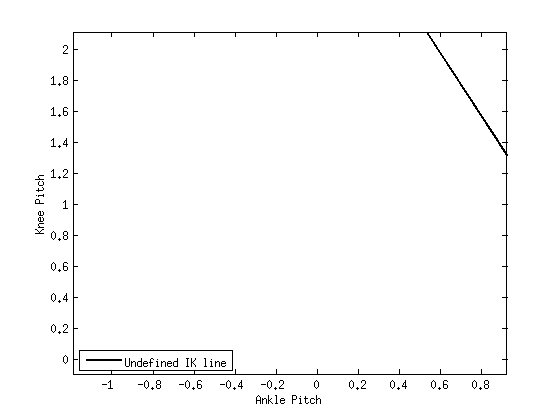
\includegraphics[height = 10cm]{Figures/locus.png}
 		\caption{Undefined Locus For Legs}
 		\label{fig:unlocus}
	\end{center}
\end{figure}\\
Now we can reconstruct and remove the rotation at the end and the transformation from ankle pitch to ankle roll from the chain to make it simpler:
\[
T_{\text{llegRotated}'} = T_\text{llegRotated}\left(T^6_5R_z\left(\pi\right)R_y(-\tfrac{\pi}{2})\right)^{-1}
\]
\[
T_{\text{llegInv}'} = \left( T_{\text{llegRotated}'} \right) ^{-1}
\]
Now we have $p_x = T_{\text{llegInv}'(1,4)}$, $p_y = T_{\text{llegInv}'(2,4)}$ and $p_z = T_{\text{llegInv}'(3,4)}$. From the new symbolic transformation matrix we have:
\begin{small}
\begin{align*}
&r_{14} = l_2\cos\theta_5 + l_1\left(\cos\theta_5\cos\theta_4 - \sin\theta_5\sin\theta_4\right)\\
&r_{24} = -l_2\sin\theta_5 - l_1\left(\sin\theta_5\cos\theta_4 + \cos\theta_5\sin\theta_4\right)\\
&r_{34} = 0
\end{align*}
\end{small}\\
We only need the translation part to extract $\theta_5$, so:
\begin{small}
\begin{align*}
&\cos\theta_5\left(l_2+l_1\cos\theta_4\right) = p_x + l_2\sin\theta_5\sin\theta_4 & \Leftrightarrow\\
&\cos\theta_5 = \cfrac{p_x + l_1\sin\theta_5\sin\theta_4}{l_2+l_1\cos\theta_4}&\text{if }l_2+l_1\cos\theta_4\neq0\\
\end{align*}
\end{small}\\
The \(l_2+l_1\cos\theta_4\) is zero if and only if \(\cos\theta_4 = 1.029\). So it is always greater than zero, because \(-1 \leq \cos \leq 1\):
\begin{small}
\begin{align*}
&\sin\theta_5\left(-l_2-l_1\cos\theta_4\right) - l_2\cos\theta_5\sin\theta_4 = p_y& \Leftrightarrow\\
&\sin\theta_5\left(-l_2-l_1\cos\theta_4\right) - l_2\cfrac{p_x + l_1\sin\theta_5\sin\theta_4}{l_2+l_1\cos\theta_4}\sin\theta_4\ =p_y & \Leftrightarrow\\
&-\sin\theta_5\left(l_2+l_1\cos\theta_4\right) - \cfrac{l_2p_x\sin\theta_4}{l_2+l_1\cos\theta_4} - \cfrac{-{l_2}^2\sin\theta_5\sin^2\theta_4}{l_2+l_1\cos\theta_4} = p_y&\Leftrightarrow\\
&-\sin\theta_5\left(l_2+l_1\cos\theta_4\right)^2 - {l_2}^2\sin\theta_5\sin^2\theta_4 = p_y\left(l_2+l_1\cos\theta_4\right) + l_2p_x\sin\theta_4 & \Leftrightarrow\\
&\theta_5 = \arcsin\left(-\frac{p_y\left(l_2+l_1\cos\theta_4\right) + l_1p_x\sin\theta_4}{{l_1}^2\sin^2\theta_4 + \left(l_2 + l_1\cos\theta_4\right)}\right)
\end{align*}
\end{small}\\
We can do the division because ${l_1}^2\sin^2\theta_4 + \left(l_2 + l_1\cos\theta_4\right)^2$ is obviously greater than zero. 
Now we can remove the two transformations of $\theta_4$ and $\theta_5$ from the symbolic matrix and then we will have a transformation matrix that is a rotation matrix:

\[
T_{\text{llegRotated}''} = T_{\text{llegRotated}'}\left(T^4_3T^5_4\right)^{-1}
\]
\[
T_{\text{llegInv}''} = \left(T_{\text{llegRotated}''}\right)^{-1}
\]
And the rotation part is:
\begin{small}
\begin{align*}
&r_{11} = \cos\theta_1\cos\theta_2\cos\theta_4 - \sin\theta_1\sin\theta_3\\
&r_{12} = -\cos\theta_3\sin\theta_1 - \cos\theta_1\cos\theta_2\sin\theta_3\\
&r_{13} = \cos\theta_1\sin\theta_2 \\
&r_{21} = -\cos\theta_3\sin\theta_2\\
&r_{22} = \sin\theta_2\sin\theta_3\\
&r_{23} = \cos\theta_2\\
&r_{31} = -\cos\theta_2\cos\theta_3\sin\theta_1 - \cos\theta_1\sin\theta_3\\
&r_{32} = -\cos\theta_1\cos\theta_3 + \cos\theta_2\sin\theta_1\sin\theta_3\\
&r_{33} = -\sin\theta_1\sin\theta_2
\end{align*}
\end{small}\\
Finally we can extract, from the transformation matrix, the remaining three angles:
\begin{small}
\begin{align*}
\theta_2 &= \arccos T_{\text{llegInv}''(2,3)}\\
\theta_2 &= \theta_2 - \cfrac{\pi}{4}\\
\theta_3 &= \arcsin\left(\cfrac{T_{\text{llegInv}''(2,2)}}{\sin\left(\theta_2+\frac{\pi}{4}\right)}\right)\\
\theta_1 &= \arccos\left(\cfrac{T_{\text{llegInv}''(3,3)}}{\sin\left(\theta_2+\frac{\pi}{4}\right)}\right)\\
\theta_1 &= \theta_1 + \cfrac{\pi}{2}
\end{align*}
\end{small}\\
The equations above don't have any problem with division by zero because of the restriction of NAO. The HipRoll joint \((\theta_2)\) doesn't reach \(-\frac{\pi}{4}\) or \(\frac{3\pi}{4}\) so the denominator never becomes zero. Finally, we will do a forward validation step for all possible set of angles.\\
Below there are all the equations of inverse kinematics for the left leg:
\begin{small}
\begin{flalign*}
T_\text{llegInv} &= \left(R_x(\tfrac{\pi}{4})\left(\left(A^0_\text{Base}\right)^{-1} T_\text{lleg} \left(A^\text{End}_6\right)^{-1}\right)\right)^{-1} \\
\theta_4 &=\pi - \arccos\left(\frac{{l_1}^2 + {l_2}^2 - \sqrt{\left(s_x-p_x\right)^2 + \left(s_y-p_y\right)^2 + \left(s_z-p_z\right)^2}^2}{2 l_1 l_2}\right) \\
\theta_6 &= \arctan\left(\frac{p_y}{p_z}\right)\quad\quad\quad\text{if} \left(l_2\cos\theta_5 + l_1 \cos\left(\theta_4 + \theta_5\right)\right) \neq 0 \\
T_{\text{llegInv}'} &= \left(\left(T_\text{llegInv}\right)^{-1}\left(T^6_5R_z\left(\pi\right)R_y(-\tfrac{\pi}{2})\right)^{-1}\right)^{-1} \\
\theta_5 &= \arcsin\left(-\frac{p_y\left(l_2+l_1\cos\theta_4\right) + l_1p_x\sin\theta_4}{{l_1}^2\sin^2\theta_4 + \left(l_2 + l_1\cos\theta_4\right)}\right) \\
\theta_5 &= \pi - \arcsin\left(-\frac{p_y\left(l_2+l_1\cos\theta_4\right) + l_1p_x\sin\theta_4}{{l_1}^2\sin^2\theta_4 + \left(l_2 + l_1\cos\theta_4\right)}\right)\\
T_{\text{llegInv}''} &= \left(\left(T_{\text{llegInv}'}\right)^{-1}\left(T^4_3T^5_4\right)^{-1}\right)^{-1} \\
\theta_2 &= \pm\arccos T_{\text{llegInv}''(2,3)} - \cfrac{\pi}{4} \\
\theta_3 &= \arcsin\left(\cfrac{T_{\text{llegInv}''(2,2)}}{\sin\left(\theta_2+\frac{\pi}{4}\right)}\right) \\
\theta_3 &= \pi - \arcsin\left(\cfrac{T_{\text{llegInv}''(2,2)}}{\sin\left(\theta_2+\frac{\pi}{4}\right)}\right) \\
\theta_1 &= \pm\arccos\left(\cfrac{T_{\text{llegInv}''(3,3)}}{\sin\left(\theta_2+\frac{\pi}{4}\right)}\right) + \cfrac{\pi}{2}
\end{flalign*}
\end{small}


\subsection{Inverse Kinematics for the Right Leg}
As we mentioned before, the chains of the legs are symmetric, so we will have a similar solution for the problem as we had with the arms. The only changes are in the rotation matrix that we use to rotate the HipYawPitch joint. Now we must rotate by $-\frac{\pi}{4}$.
\[
T_{\text{rleg}} = A^0_\text{Base}T^1_0T^2_1T^3_2T^4_3T^5_4T^6_5R_z(\pi)R_y(-\tfrac{\pi}{2})A^\text{End}_6
\]
\[
T_{\text{rleg}'} = T_\text{rleg}{\left(A^\text{End}_6\right)}^{-1}
\]
\[
T_{\text{rleg}''} = {\left(A^0_\text{Base}\right)}^{-1}T_{\text{rleg}'}
\]
\[
T_\text{rlegRotated} = R_x(-\tfrac{\pi}{4}) T_{\text{rleg}''}
\]
\[
T_\text{rlegInv} = {\left(T_\text{rlegRotated}\right)}^{-1}
\]
After that, the symbolic matrix for the right leg is exactly the same as the symbolic matrix for the left leg. From this point of view, if we follow all the steps as we did with the left leg, we will conclude to the same equations. So, the final equations are:
\begin{small}
\begin{flalign*}
T_\text{rlegInv} &= \left(R_x(\tfrac{\pi}{4})\left(\left(A^0_\text{Base}\right)^{-1} T_\text{rleg} \left(A^\text{End}_6\right)^{-1}\right)\right)^{-1} \\
\theta_4 &=\pi - \arccos\left(\frac{{l_1}^2 + {l_2}^2 - \sqrt{\left(s_x-p_x\right)^2 + \left(s_y-p_y\right)^2 + \left(s_z-p_z\right)^2}^2}{2 l_1 l_2}\right) \\
\theta_6 &= \arctan\left(\frac{p_y}{p_z}\right)\quad\quad\quad\text{if} \left(l_2\cos\theta_5 + l_1 \cos\left(\theta_4 + \theta_5\right)\right) \neq 0 \\
T_{\text{rlegInv}'} &= \left(\left(T_\text{rlegInv}\right)^{-1}\left(T^6_5R_z\left(\pi\right)R_y(-\tfrac{\pi}{2})\right)^{-1}\right)^{-1} \\
\theta_5 &= \arcsin\left(-\frac{p_y\left(l_2+l_1\cos\theta_4\right) + l_1p_x\sin\theta_4}{{l_1}^2\sin^2\theta_4 + \left(l_2 + l_1\cos\theta_4\right)}\right) \\
\theta_5 &= \pi - \arcsin\left(-\frac{p_y\left(l_2+l_1\cos\theta_4\right) + l_1p_x\sin\theta_4}{{l_1}^2\sin^2\theta_4 + \left(l_2 + l_1\cos\theta_4\right)}\right)\\
T_{\text{rlegInv}''} &= \left(\left(T_{\text{rlegInv}'}\right)^{-1}\left(T^4_3T^5_4\right)^{-1}\right)^{-1} \\
\theta_2 &= \pm\arccos T_{\text{rlegInv}''(2,3)} + \cfrac{\pi}{4} \\
\theta_3 &= \arcsin\left(\cfrac{T_{\text{rlegInv}''(2,2)}}{\sin\left(\theta_2 - \frac{\pi}{4}\right)}\right) \\
\theta_3 &= \pi - \arcsin\left(\cfrac{T_{\text{rlegInv}''(2,2)}}{\sin\left(\theta_2 - \frac{\pi}{4}\right)}\right) \\
\theta_1 &= \pm\arccos\left(\cfrac{T_{\text{rlegInv}''(3,3)}}{\sin\left(\theta_2 - \frac{\pi}{4}\right)}\right) + \cfrac{\pi}{2}
\end{flalign*}
\end{small}

\subsection{Undefined Target Points For Legs}
\label{undefined}
As we mentioned before, we have some target points for which we can't find an inverse kinematics solution. These target points are presented in the figure~\ref{fig:undefined}, alongside with all the values of the angles that are responsible for this singularity. As we can see, we let the robot to do a lot of movements in the field, and none of those movements was close to the points of the singularity. In real world, it is very rare for someone to give target points in that area. Also, when someone is executing a trajectory, they ''feed'' inverse kinematics with a lot of target points per second (usually they provide inverse kinematics with target points with frequency 50 to 100 Hz), so if one of those target points is in the area of singularity, we will find a solution for the next target point. Because we are working in high frequency rate, the singularity will be unnoticed and the movement will be continued normally.
\begin{figure}[h]
	\begin{center}
		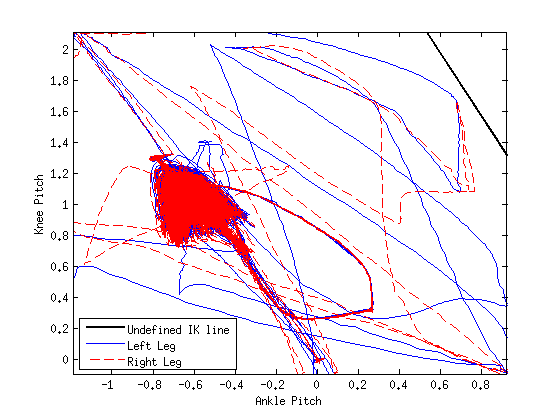
\includegraphics[height = 10cm]{Figures/undefined.png}
 		\caption{Undefined Target Points For Legs}
 		\label{fig:undefined}
	\end{center}
\end{figure}


\section{Implementation}
Now that we have all the equations for both problems, we must integrate them in the code of the team. The code of the team is written in \verb!C++! so because \verb!C++! doesn't have any library for fast linear algebra operations, we must develop a minimalistic matrix framework. Then, using this framework, we must write some functions that will implement the equations of forward and inverse kinematics in \verb!C++!.
\subsection{KMat: Kouretes Math Library}
KMat is a library developed by Emmanouil Orfanoudakis~\cite{orfanoudakis2011} that supports a strict subset of algebraic operations. The focus of the library is mainly in real numbers operations and the primary goal of KMat is low memory footprint and calculation efficiency. The typical linear algebra libraries do run-time validation for the compatibility of the operands and are optimized for large matrices. On the other hand, KMat is optimized for small matrices (typically \((3\times3)\) or \((4\times4)\)) and only a subset of operations (addition, subtraction, multiplication, scalar addition, scalar multiplication, transposition, inversion) have been implemented. KMat supports two type of matrices: Dense matrices and Affine transformation matrices.\\
For our work we used mainly the affine type of matrices and we expanded the functions of the library with some functions that are extremely useful for the kinematics computations. These functions are some initialization functions that initialize a matrix with the given DH parameters or reconstruct of the matrix given the target points etc.
\subsection{Nao Kinematics in C++}
Along with KMat we created two more libraries ForwardKinematics and InverseKinematics. ForwardKinematics has the functions to calculate the location of an end effector of a kinematic chain, given the joint values for this chain. The union of independent chains with common base frame is possible, so someone can take the position of the top camera relatively to one of the legs. Finally, we have a function to calculate the center of mass of the robot. The input of each function is the values of the joints with the order that they appear in the kinematic chains.\\
The inverse kinematics library has five functions, each of which solves the problem for a kinematic chain. All functions take, as input, the position and the orientation of the target point and the output is the values of the joints, for all the possible solutions for this point. It is possible to have a solution with two set of values and then the user can decide what output will be used. \\
As we mentioned before, the legs have one common joint (HipYawPitch) but if we give two target points, one for each leg, inverse kinematics for the left leg will most likely  return a different value for this joint than the inverse kinematics for the right leg. We must decide what value will be set to the HipYawPitch joint and one solution to this problem is to make the support leg (the leg that keeps the robot in balance) the master of this joint or another solution is to get the mean of these two values. Both solutions are not perfect but with a large probability, if we design trajectories carefully, the resulted values from inverse kinematics for this joint will be close enough. Thus, we can use any of these two solutions and the result will be similar to the result if the joint was independent.

% ------------------------------------------------------------------------
%%% Local Variables:
%%% mode: latex
%%% TeX-master: "../thesis"
%%% End:vides a simple interface with two methods the in and read. \tt{Read} returns the requested data , on the other hand \tt{in} first remove the data and then returns them to the module. The requests for data have the following form robot[x].publisher.type_of_message. Blackboard's transparent interface enables the user to access 